\newpage
\section{Transformatormodell}


\subsection{Idealer Transformator}

\begin{minipage}[t]{0.4\columnwidth}
    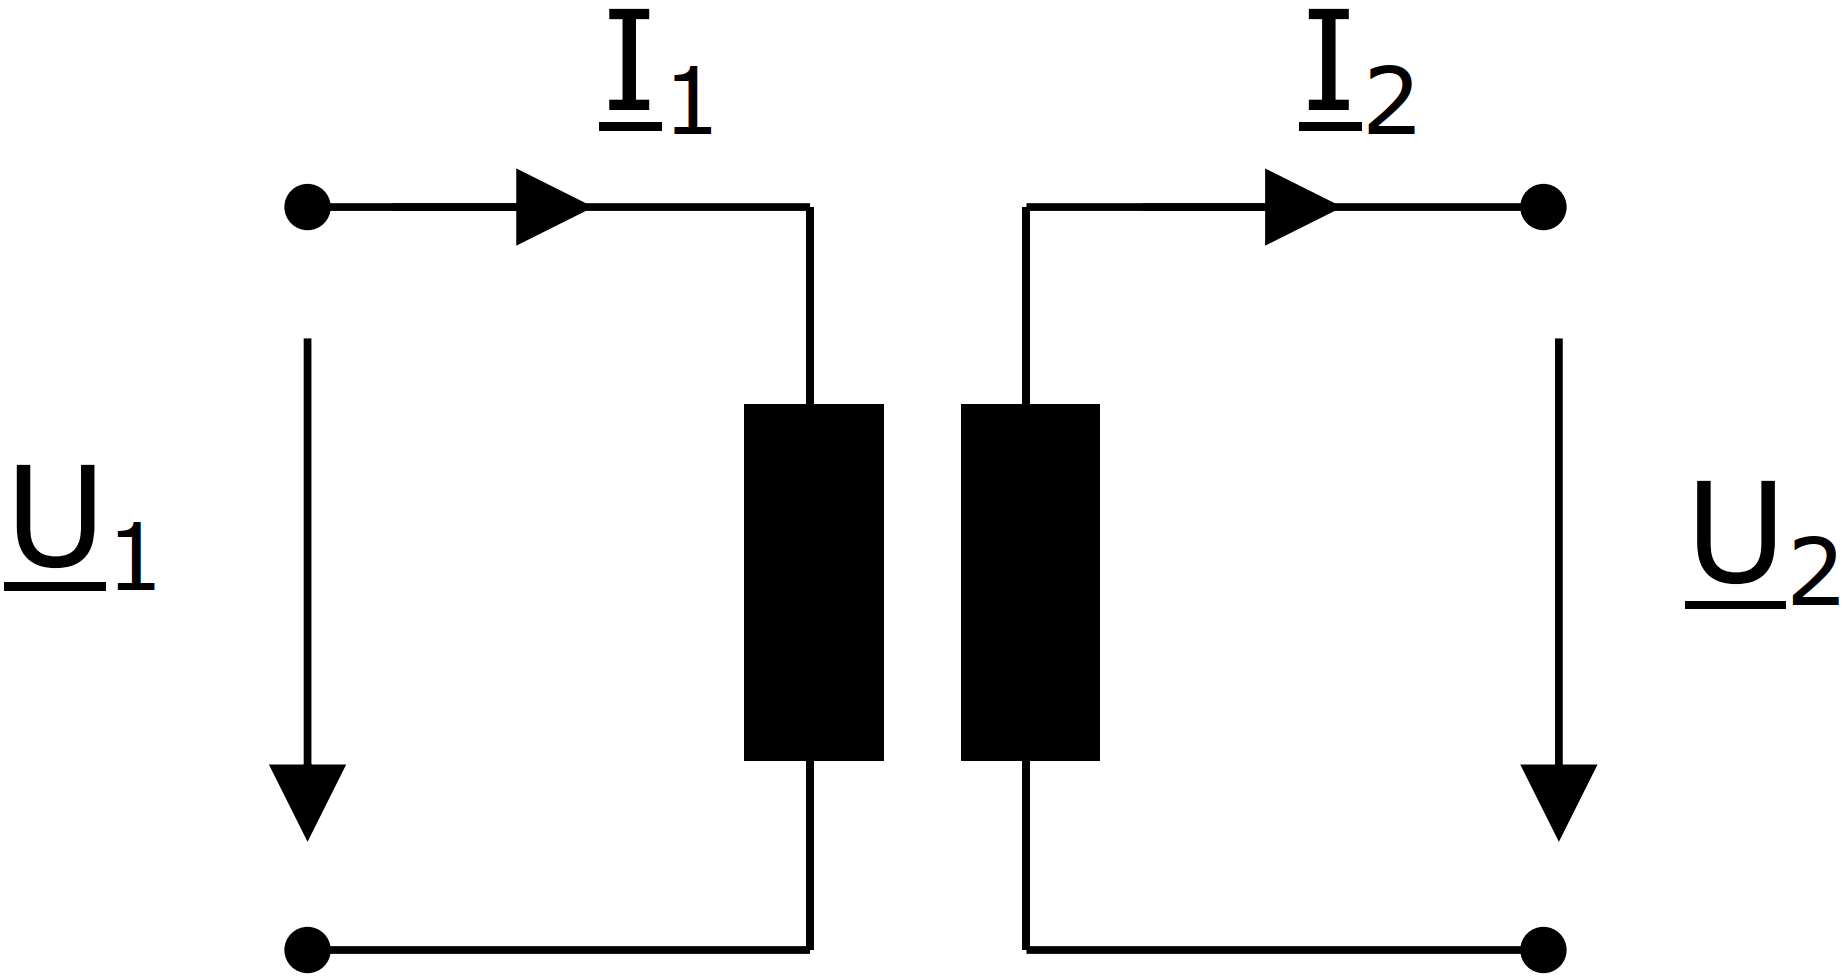
\includegraphics[width=0.8\columnwidth, align=c]{images/Idealer_Transformator_1.png}
\end{minipage}
\hfill
\begin{minipage}[t]{0.58\columnwidth}
    $
        \boxed{\frac{\underline{U_1}}{\underline{U_2}} = \frac{\underline{I_2}}{\underline{I_1}} = t}
    $
\end{minipage}



\subsection{Reales Transformatormodell}

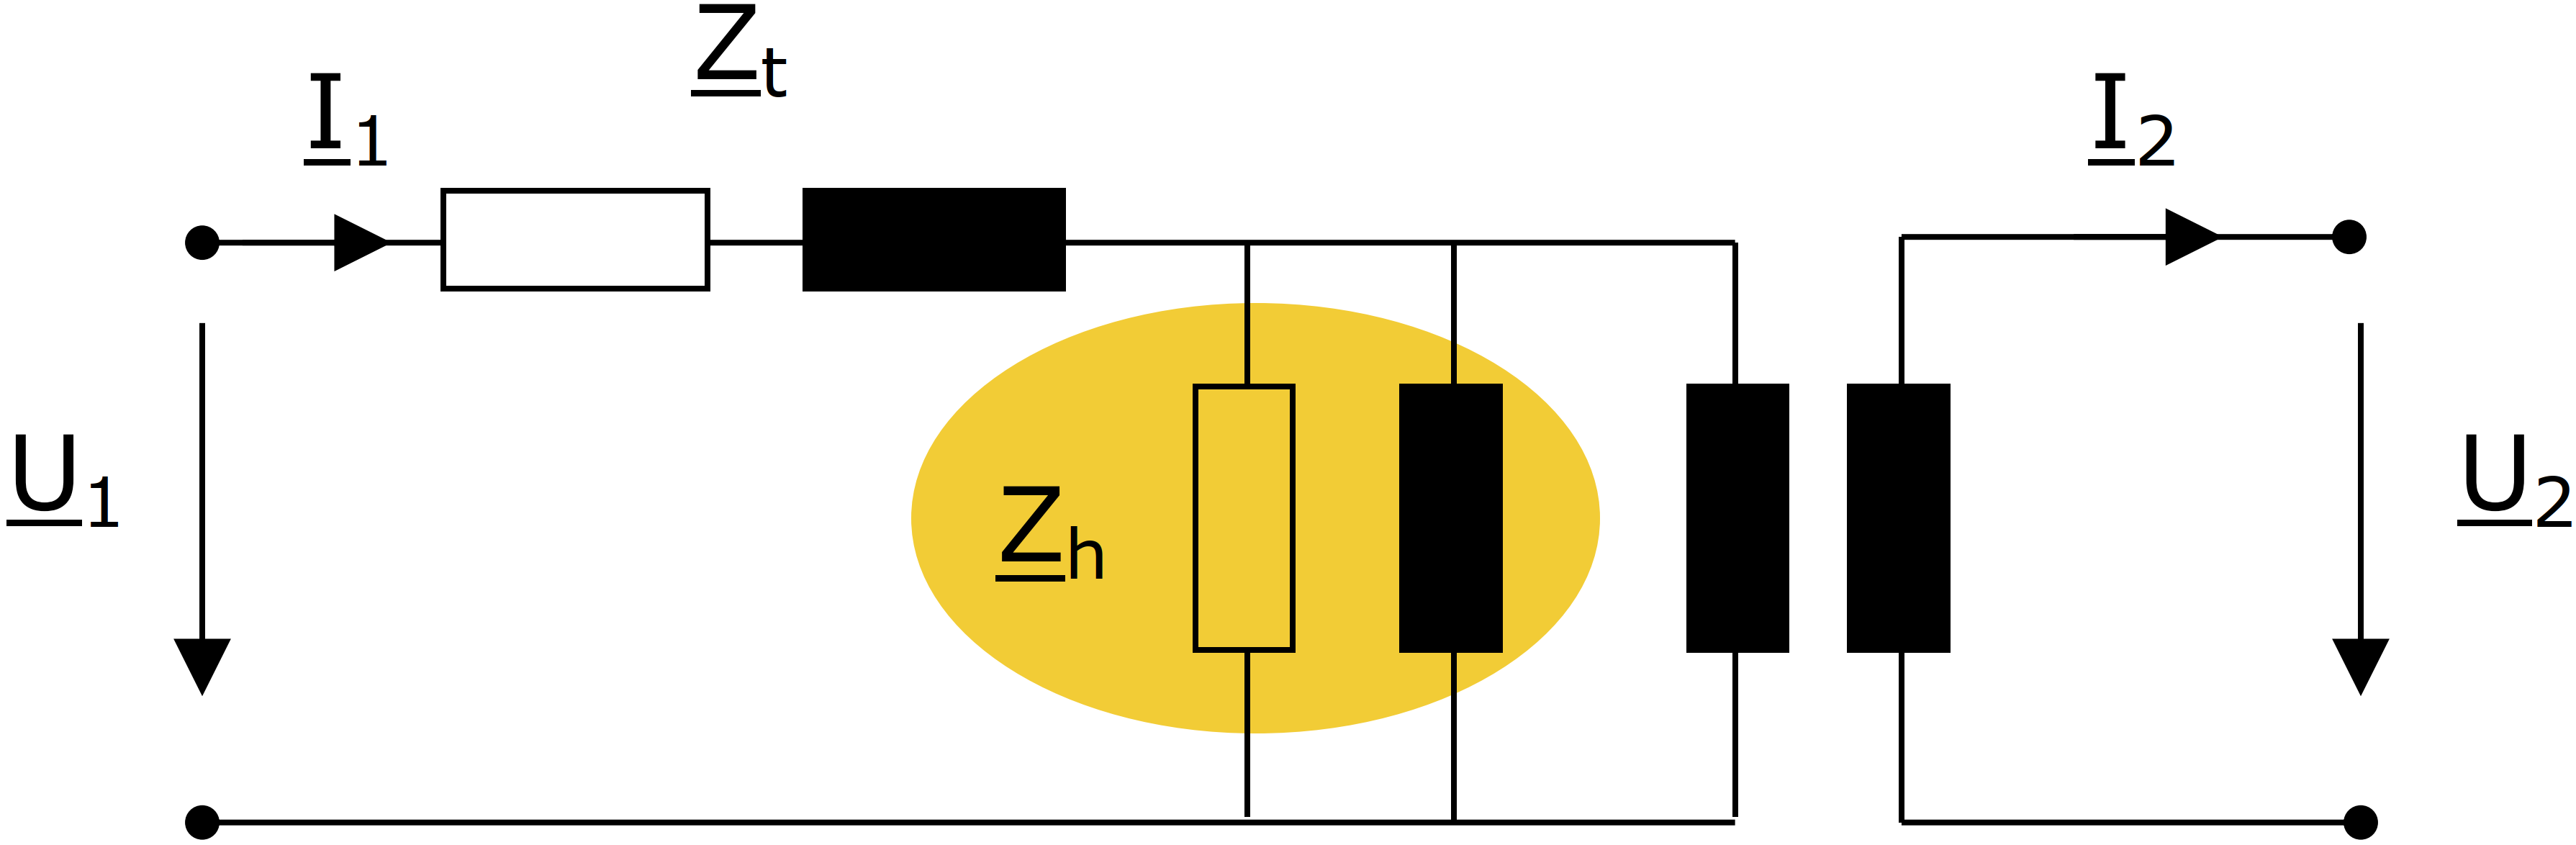
\includegraphics[width=0.98\columnwidth, align=c]{images/Reales_Transformatorbild_1.png}

\vspace{0.15cm}

\begin{itemize}
    \item Streuverluste
    \item Wicklungsverluste
    \item Kernverluste
\end{itemize}


\subsection{Praktisches Transformatormodell}

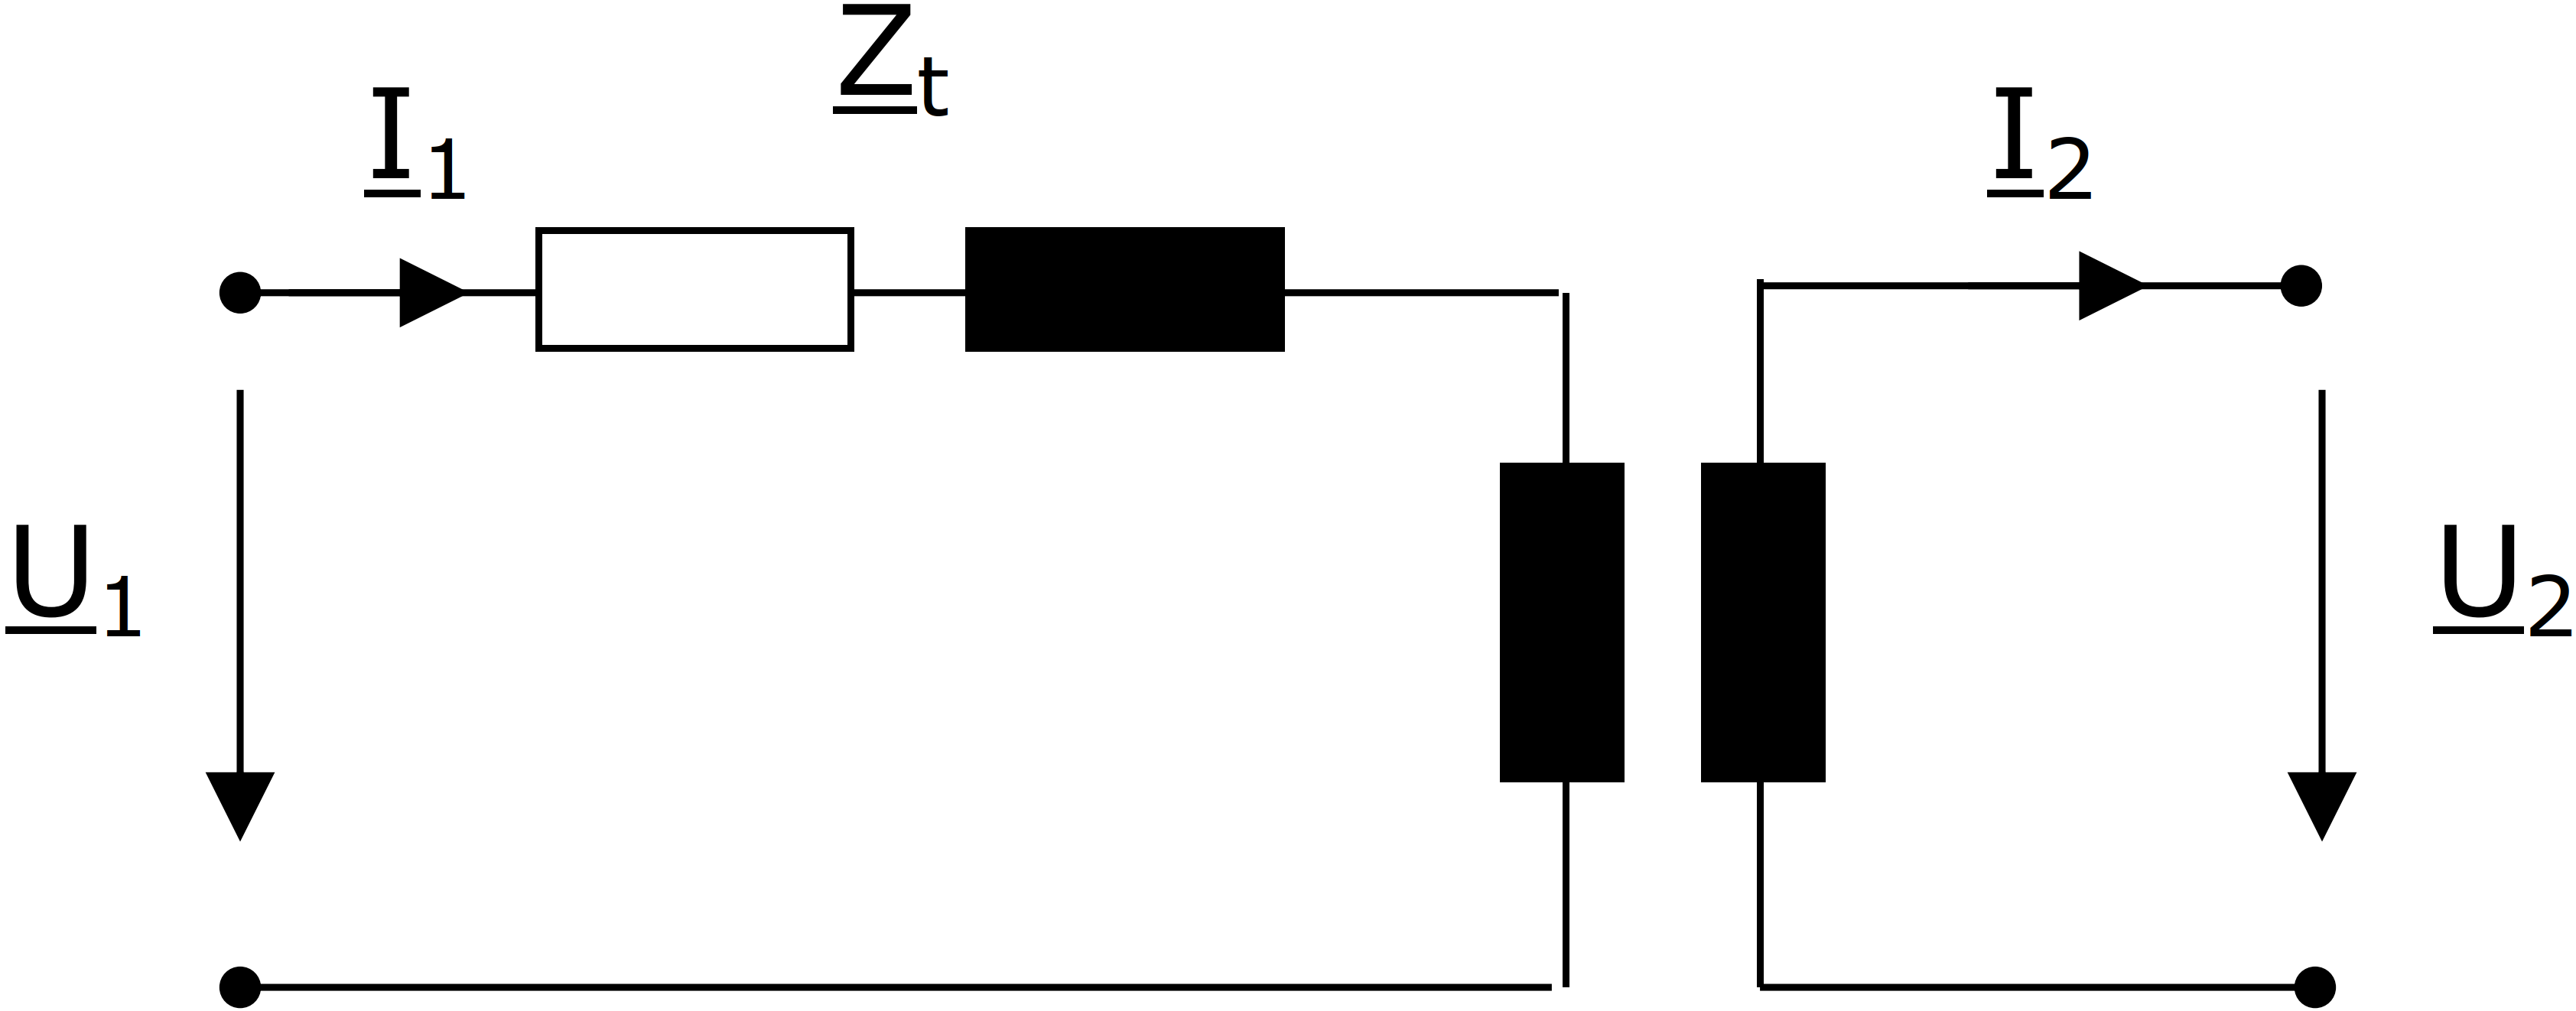
\includegraphics[width=0.98\columnwidth, align=c]{images/Praktisches_Transformatorbild_2.png}

\vspace{0.15cm}

\begin{itemize}
    \item \( Z_h \gg Z_t \Rightarrow Z_h \) vernachlässigen
    \item \( I_h \approx \,\%\!1 \) von \( I_t \) bei großen Transformatoren
    \item Kernverluste
\end{itemize}


\subsection{Umrechnung von Impedanzen}


\begin{minipage}[t]{0.48\columnwidth}
    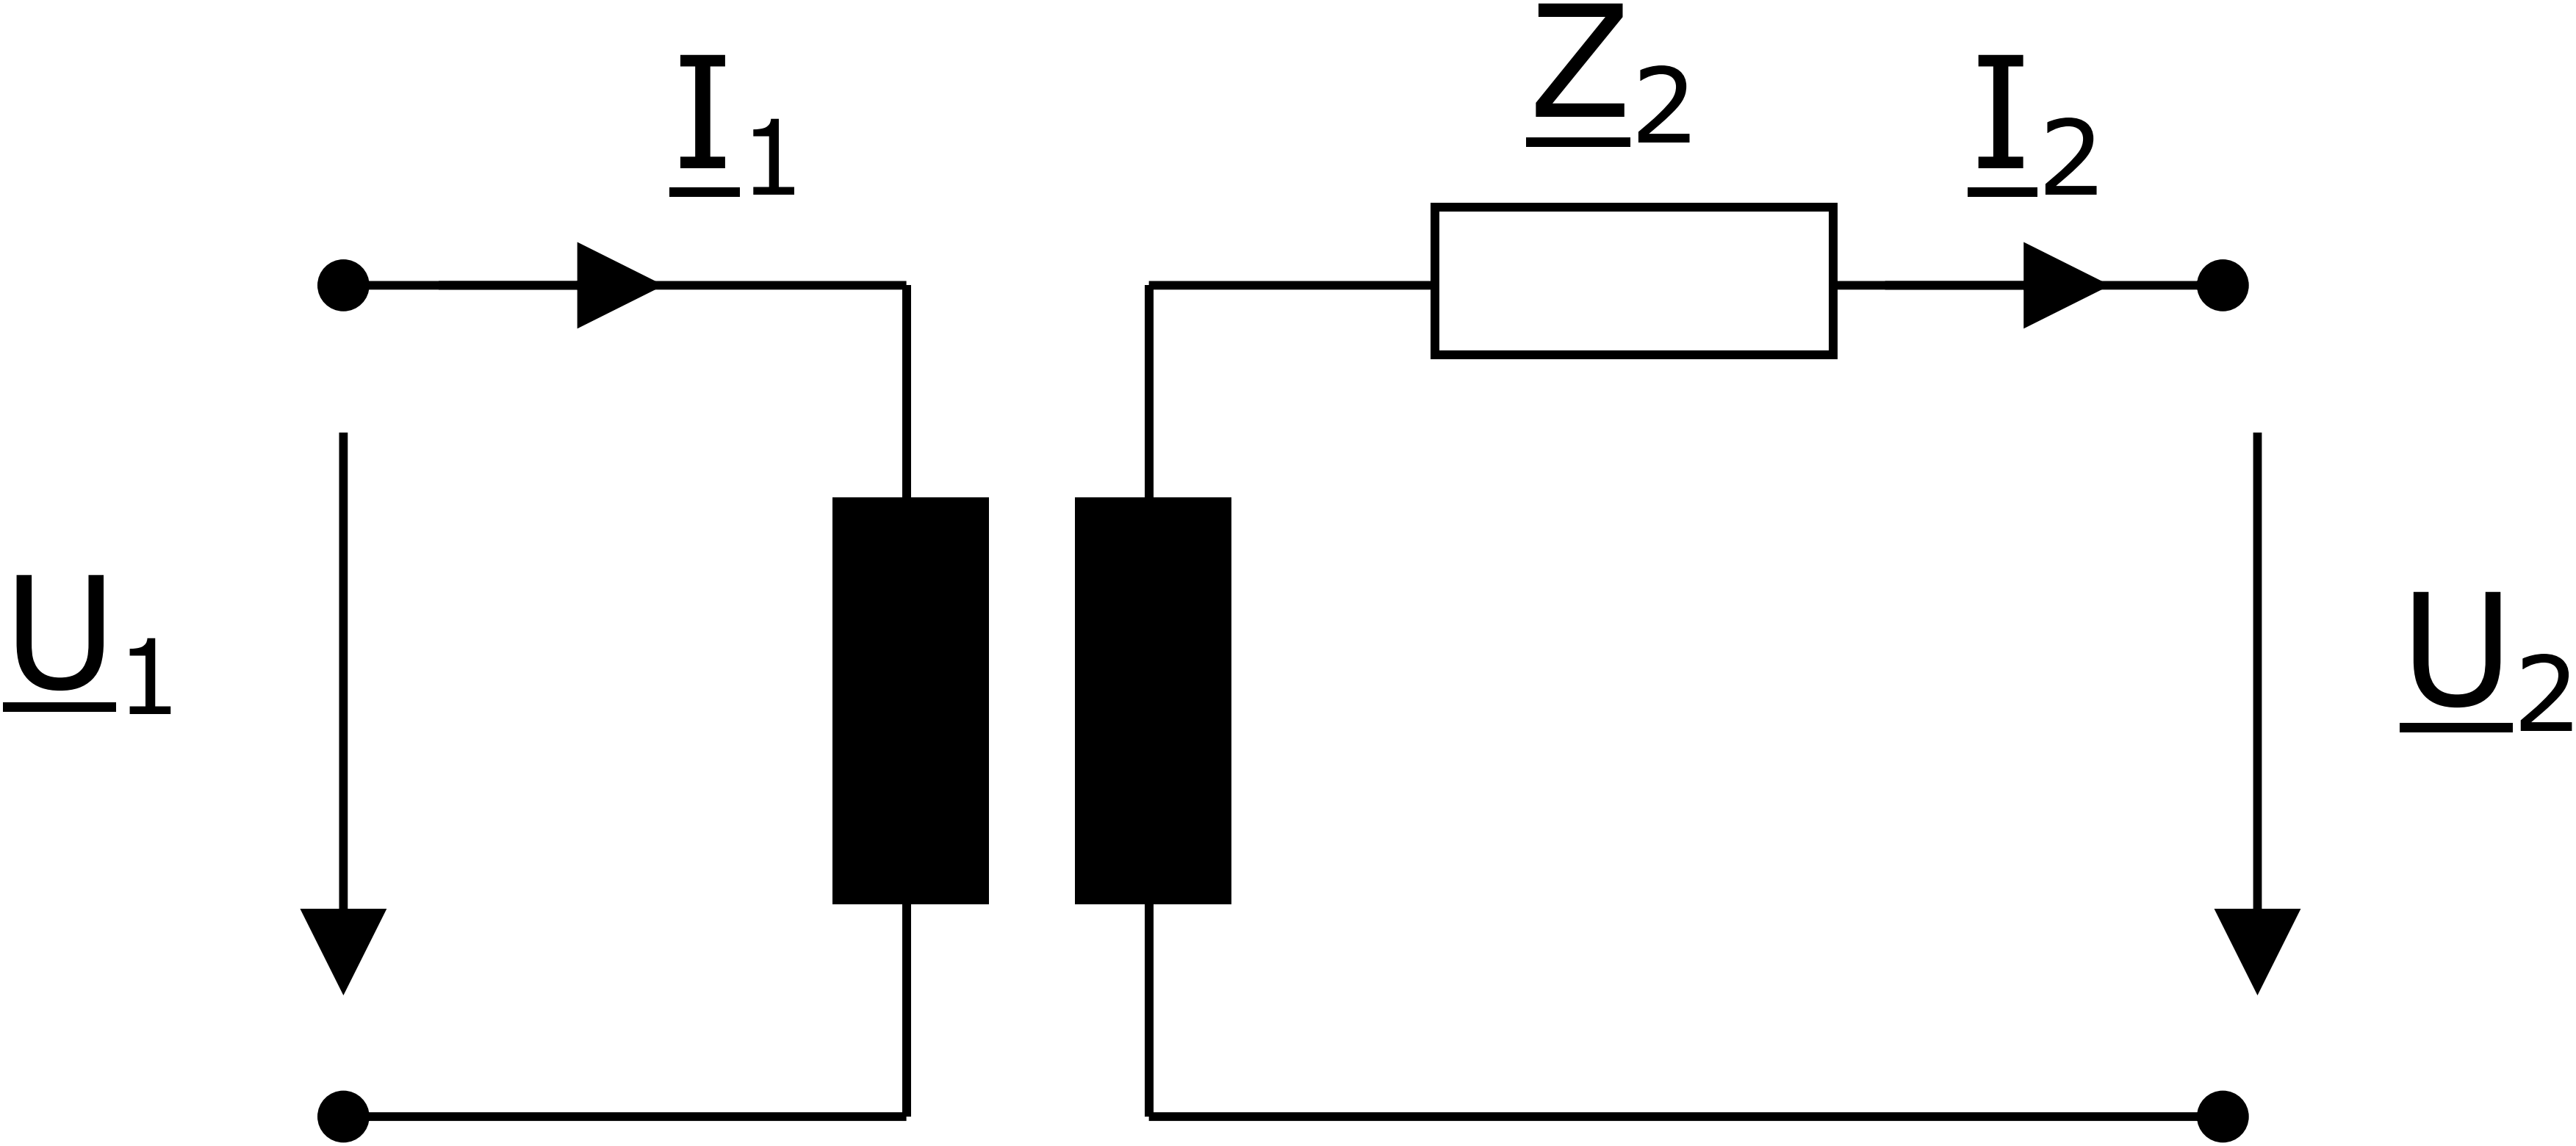
\includegraphics[width=0.98\columnwidth, align=c]{images/Umrechnung_Impedanzen_1.png}
\end{minipage}
\hfill
\begin{minipage}[t]{0.48\columnwidth}
    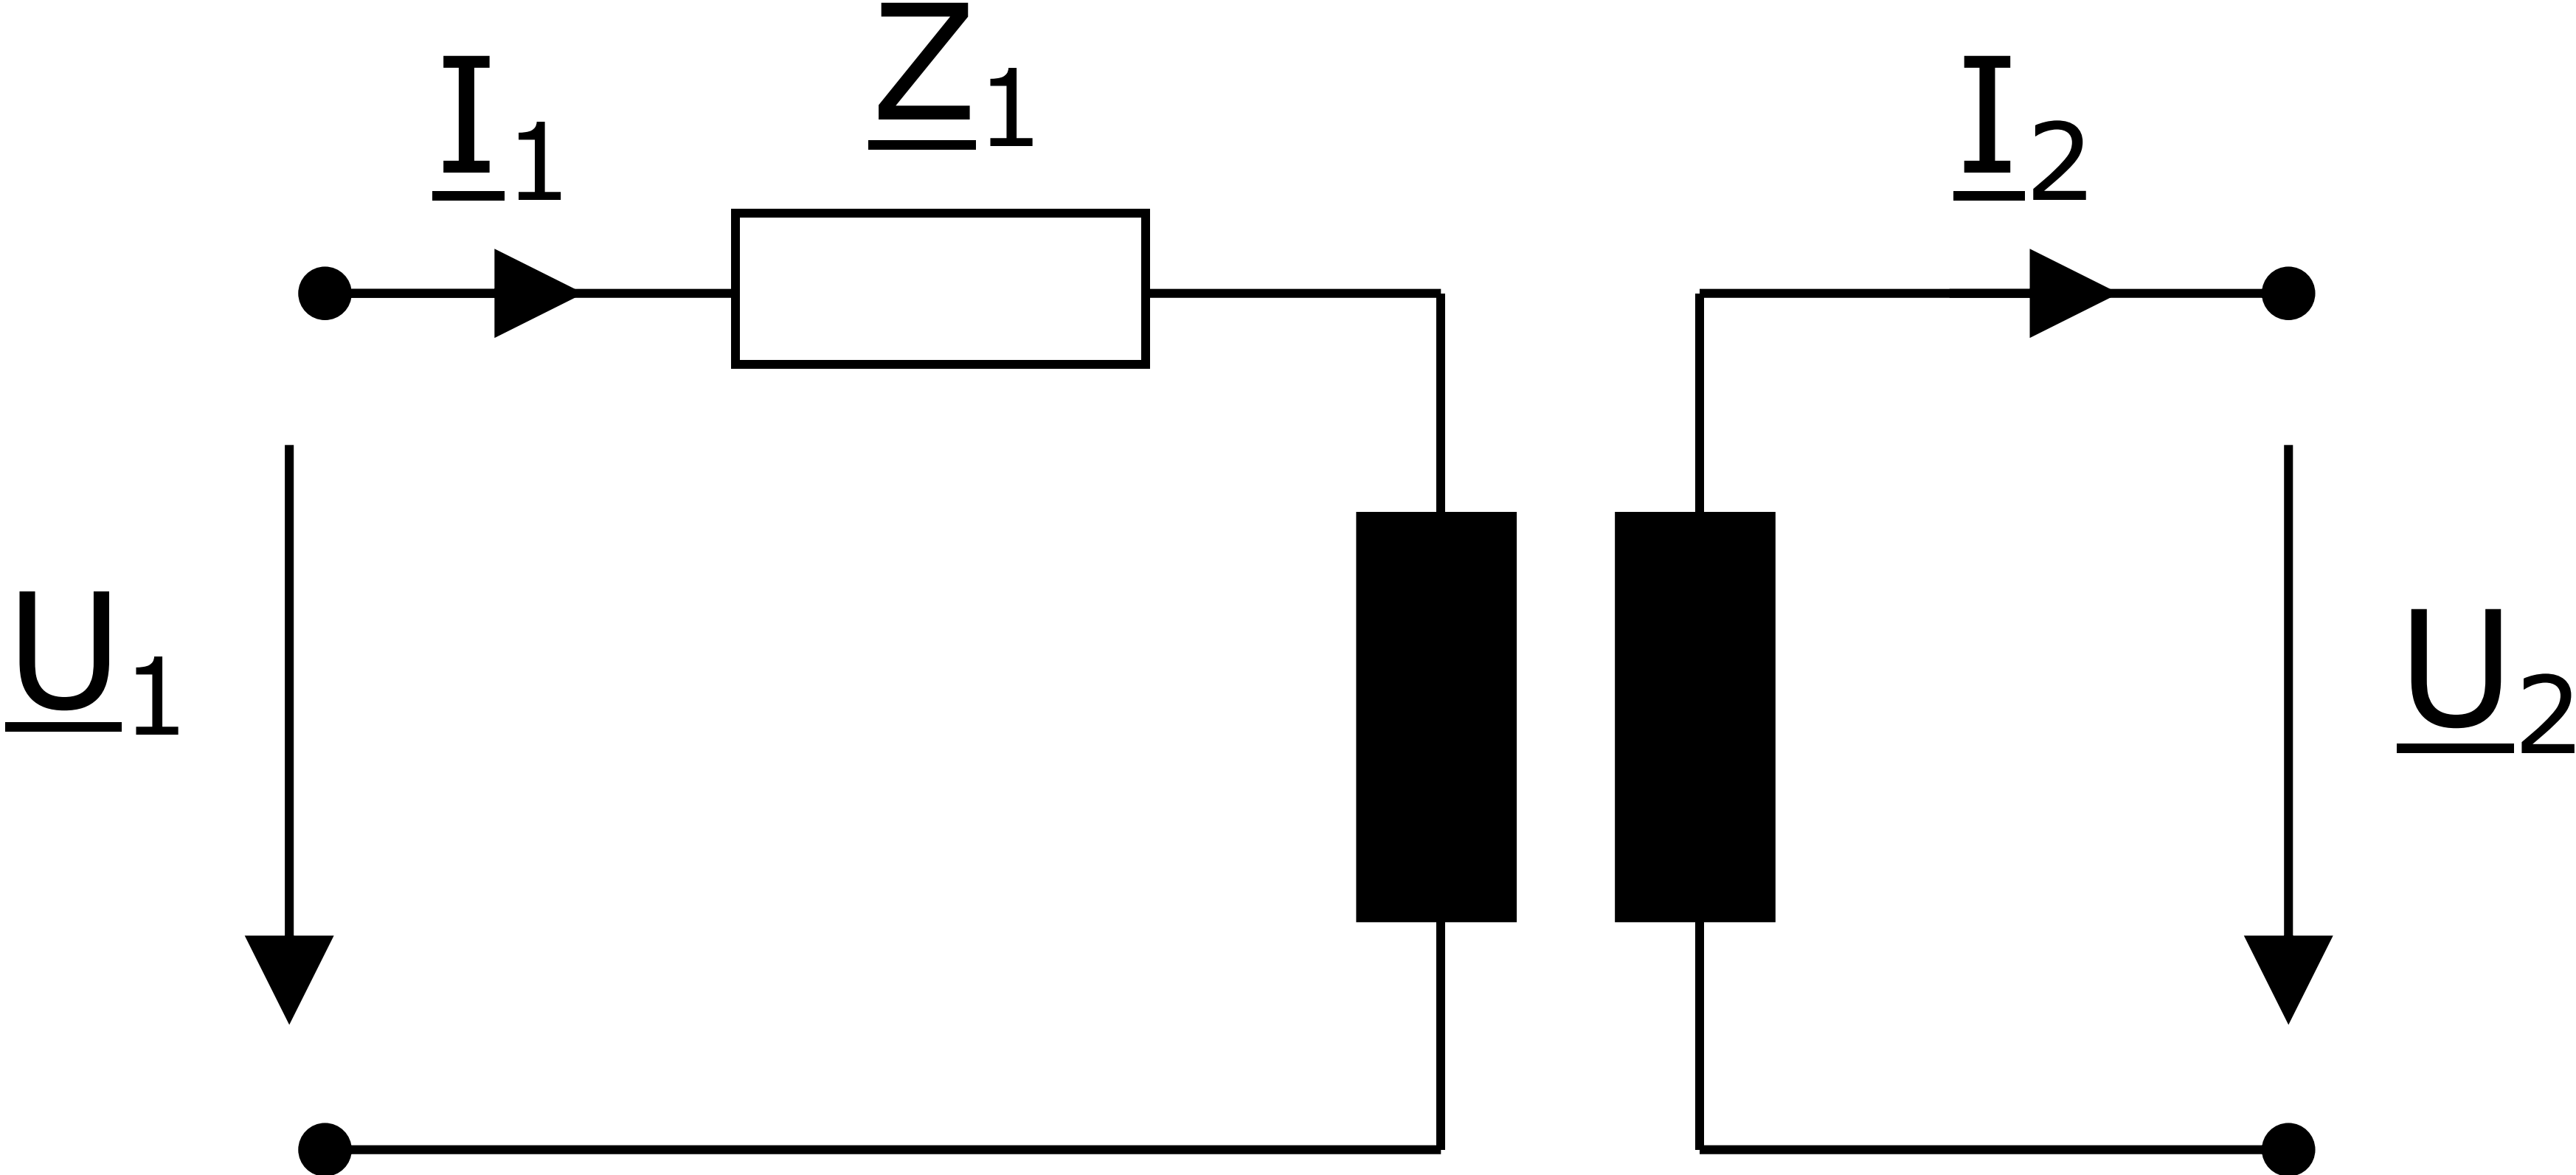
\includegraphics[width=0.98\columnwidth, align=c]{images/Umrechnung_Impedanzen_2.png}
\end{minipage}

\vspace{0.15cm}

$
    \boxed{\frac{\underline{Z_1}}{\underline{Z_2}} = t^2}
$


\subsection{Dreiphasentransformatoren}

\begin{itemize}
    \item Verschaltung der drei Phasenwicklungen auf Primär- und Sekundärseite wirkt sich auf Übersetzungsverhältnis aus.
    \item Amplitude und Phasenlage der Spannung können verändert werden.
    \item Übersetzungsverhältnis wird komplex: \( t \)
\end{itemize}

\vspace{0.15cm}

\begin{minipage}[c]{0.48\columnwidth}
    \myul{\textbf{Mögliche Schaltungen}}\\
\end{minipage}
\hfill
\begin{minipage}[c]{0.48\columnwidth}
    \myul{\textbf{Bezeichnung}}\\
\end{minipage}

\begin{minipage}[c]{0.48\columnwidth}
    \begin{itemize}
        \item Y \dots\ Sternschaltung
        \item D \dots\ Dreieck-Schaltung
        \item Z \dots\ „Zick-zack“-Schaltung
    \end{itemize}
\end{minipage}
\hfill
\begin{minipage}[c]{0.48\columnwidth}
    \begin{itemize}
        \item 1. Buchstabe (groß): \\
        Schaltung Oberspannungsseite
        \item 2. Buchstabe (klein): \\
        Schaltung Unterspannungsseite
        \item Zahl: Phasendrehung = Zahl \( \times \) 30°
    \end{itemize}
\end{minipage}

\subsection{Schaltgruppen}

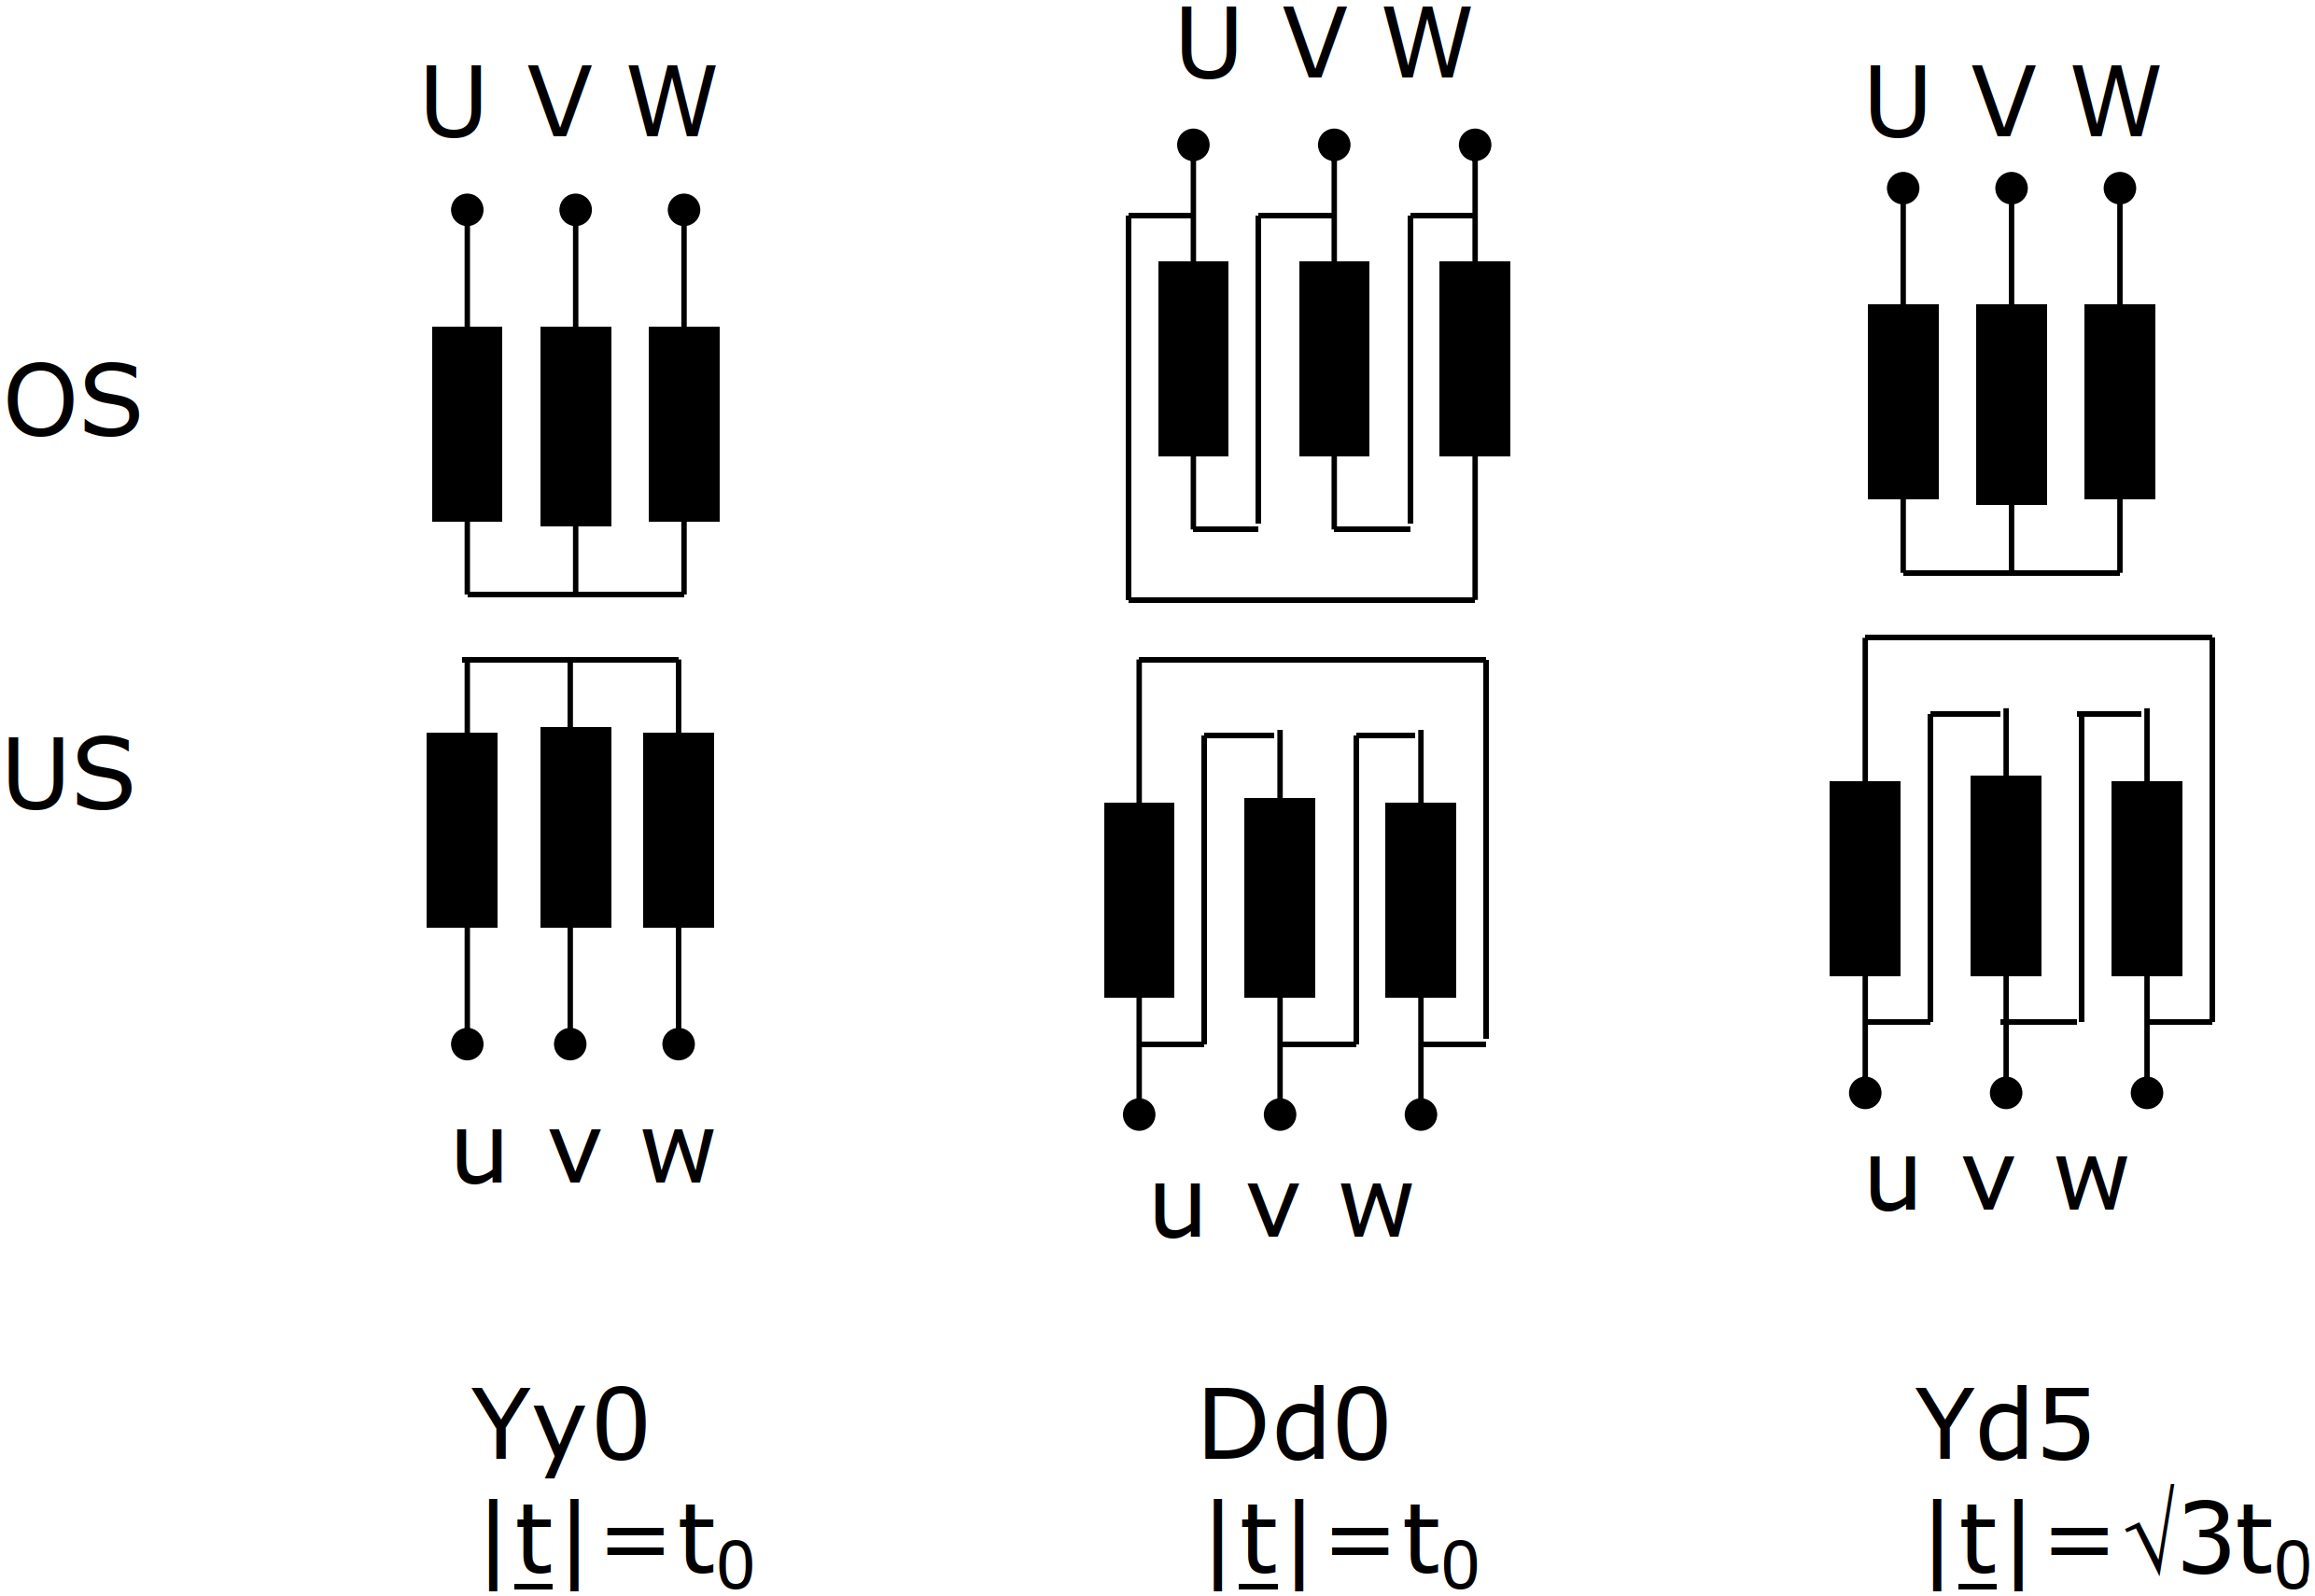
\includegraphics[width=0.75\columnwidth, align=c]{images/Schaltgruppen.png}






























